\message{ !name(main.tex)}\documentclass[12pt]{article}
%%%%%%%%%%%%%%%%%%%%%%%%%%%%%%%%%%%%%%%%%

\usepackage{amscd}
\usepackage{amsmath}
\usepackage{amssymb}
\usepackage{amsthm}


\usepackage{cite}

\usepackage{epsfig}
\usepackage{verbatim}
\usepackage{graphicx}
\usepackage{amsthm}
\pagestyle{empty}
\usepackage{color}




\title{\large\bf Directional Dipole Model for Subsurface Scattering}
\author{Pan An~(A0134556A)}

\begin{document}

\message{ !name(main.tex) !offset(83) }
\begin{figure}[!ht]
  \centering
  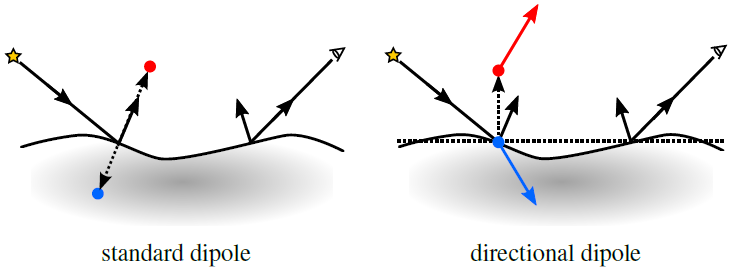
\includegraphics[scale=0.5]{dipoles.png}
  \caption{Standard dipole method(left) and directional dipole.}
  \label{fig:dipole}
\end{figure}

\message{ !name(main.tex) !offset(128) }

\end{document}

%%% Local Variables:
%%% mode: latex
%%% TeX-master: t
%%% End:
